\section*{1. Assignment 3.1}
\textbf{Read and understand the papers from Zhang and Heikkil (provided in LEA). Based on your understanding of camera calibration, design a calibration setup and detail the actual calibration process. \\
Test the provided camera on your laptop and ensure you can capture still images.}

\begin{itemize}
\item We used VLC player as a tool to capture images since we can disable the auto-focussing function that is in-built in the camera with VLC player. This is required since auto-focussing changes the focal length of the lens changes.
\end{itemize}

\section*{2. Deliverables 3.1}
\textbf{Write a design report describing the calibration process, including a theoretical part that describes the camera and lens errors measured and corrected by the calibration. Your design report should cover:}

\subsection*{1. A description of the setup for calibration, including possible pitfalls}
\begin{figure}[H]
\begin{center}
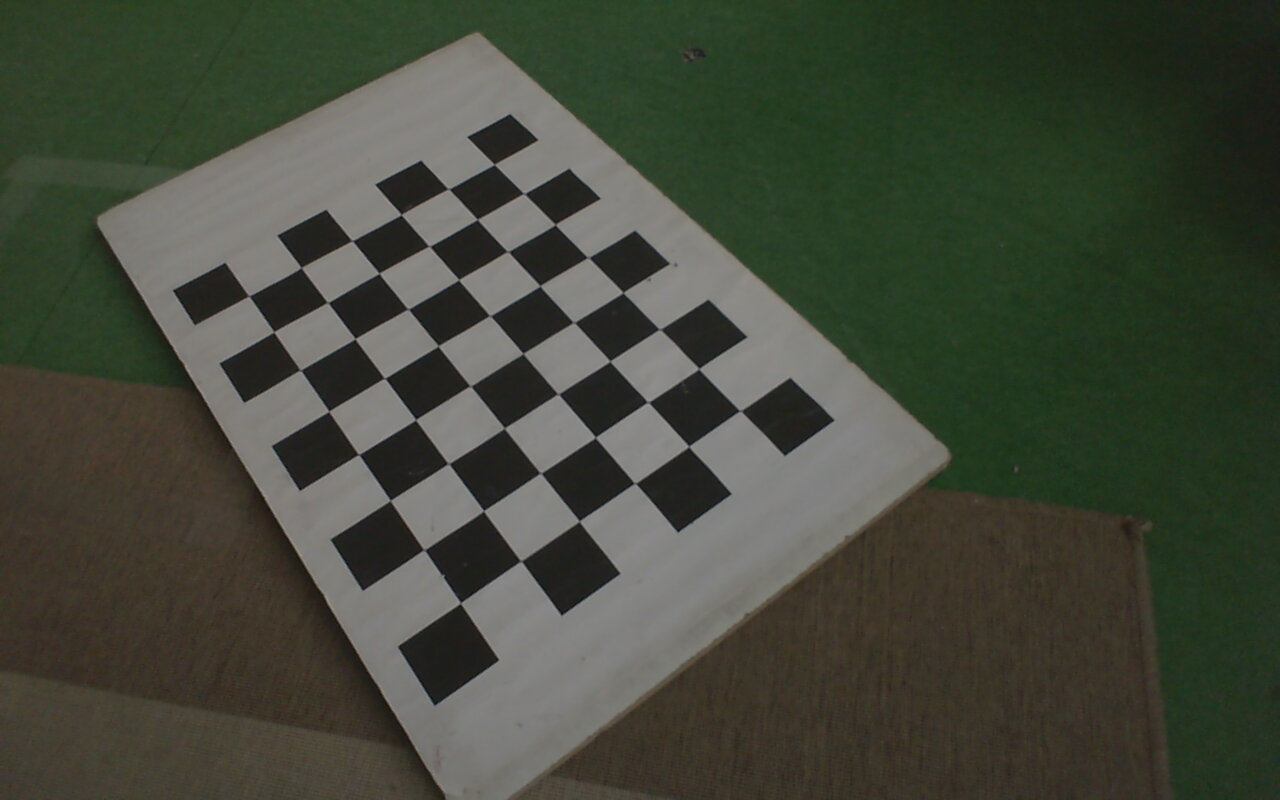
\includegraphics[width=0.7\textwidth]{data/1.jpg}
\caption{Sample image}
\label{fig:sample}
\end{center}
\end{figure}
\begin{itemize}
\item As shown in fig. \ref{fig:sample}, we place the checker board on the ground.
\item The size of the checker board was measured to be $72$ mm.
\item The provided camera is then used to take images of this checker board from multiple perspectives.
\item The poses for each image captured can be found in fig. \ref{fig:poses}.
\end{itemize}
\subsubsection*{Mathematical background}
The standard camera model calibration algorithm assumes a pinhole camera model:
\begin{equation}
w \begin{bmatrix} x & y & 1 \end{bmatrix} = \begin{bmatrix} X & Y & Z & 1 \end{bmatrix} \begin{bmatrix} R \\ t \end{bmatrix} K
\end{equation}
where,
\begin{itemize}
\item $(X,Y,Z)$ are world coordinates of a point.
\item $(x,y)$ are image coordinates of the corresponding image point in pixels.
\item $w$ is arbitrary homogeneous coordinates scale factor.
\item $K$ is the camera intrinsic matrix defined as
\begin{equation}
K = \begin{bmatrix}
f_x & 0 & 0 \\
s & f_y & 0 \\
c_x & c_y & 1
\end{bmatrix}
\end{equation} 
\begin{itemize}
\item The coordinates $(c_x, c_y)$ represent the optical center (principal point) in pixels.
\item When $x$- and $y$-axes are orthogonal to each other, the skew parameter $s$ equals $0$.
\item $f_x = F*s_x$
\item $f_y = F*s_y$
\item $F$ is the focal length in world units, typically expressed in millimeters.
\item $[s_x, s_y]$  are the number of pixels per world unit in the x and y direction respectively.
\item $f_x$ and $f_y$ are expressed in pixels.
\end{itemize}
\item $R$ rotation matrix represents the 3D rotations of the camera.
\item $t$ represents the translation of the camera relative to the world coordinate system.
\end{itemize}

\subsection*{2. An estimation of the number of images and image positions required}
\begin{itemize}
\item The \texttt{Camera Calibrator} in \texttt{MatLab} required at least 3 images for calibration.
\item It is recommended that we use at least 10-20 images for calibration so that the optimization function can converge efficiently.
\item We used 51 images. This introduces a lot of redundancy however it enables us to attain higher calibration accuracy.
\end{itemize}

\subsection*{3. A description of the parameters (what do they mean?) calculated by the Matlab calibration toolbox}
\begin{itemize}
\item The intrinsic camera matrix was evaluated to be:
\begin{equation}
K = 10^3\begin{bmatrix}
1.0018 & 0 & 0 \\
0.0028 & 1.0066 & 0 \\
0.6217 & 0.4154 & 0.0010
\end{bmatrix}
\end{equation}
\item The radial distortion was computed to be 
\begin{equation}
\begin{bmatrix}
0.0087 & 0.0619 & -0.1739
\end{bmatrix}
\end{equation}
\item The tangential distortion was computed to be 
\begin{equation}
\begin{bmatrix}
0.0029 & -6.6483 \cdot 10^{-4}
\end{bmatrix}
\end{equation}
\end{itemize}

\subsection*{4. Discuss possible problems or error sources that can disturb the calibration process. Include any observation you may have made while testing the proper functioning of the camera with your laptop}
\begin{itemize}
\item We observed that unsteady setup could introduce blur in the image. Such images are bad examples to use for calibration procedure.
\item Some devices, like the provided camera, came with built-in auto-focussing function. This is undesirable since auto-focussing changes the focal length of the lens. We cannot use pin-hole camera model for cameras with variable focal length.
\end{itemize}

\section*{3. Assignment 3.2}
\subsection*{Perform the camera calibration experiment designed in assignment 3.1. Document all relevant aspects needed to assess the quality of your obtained camera parameters.}

\section*{4. Deliverables 3.2}
\textbf{Write a report describing the calibration process, including a theoretical part that describes the camera and lens errors measured and corrected by the calibration:}
\subsection*{1. Describe the images poses used for calibration and report the found camera parameters including any error estimates (where applicable)}
\begin{figure}[H]
\begin{center}
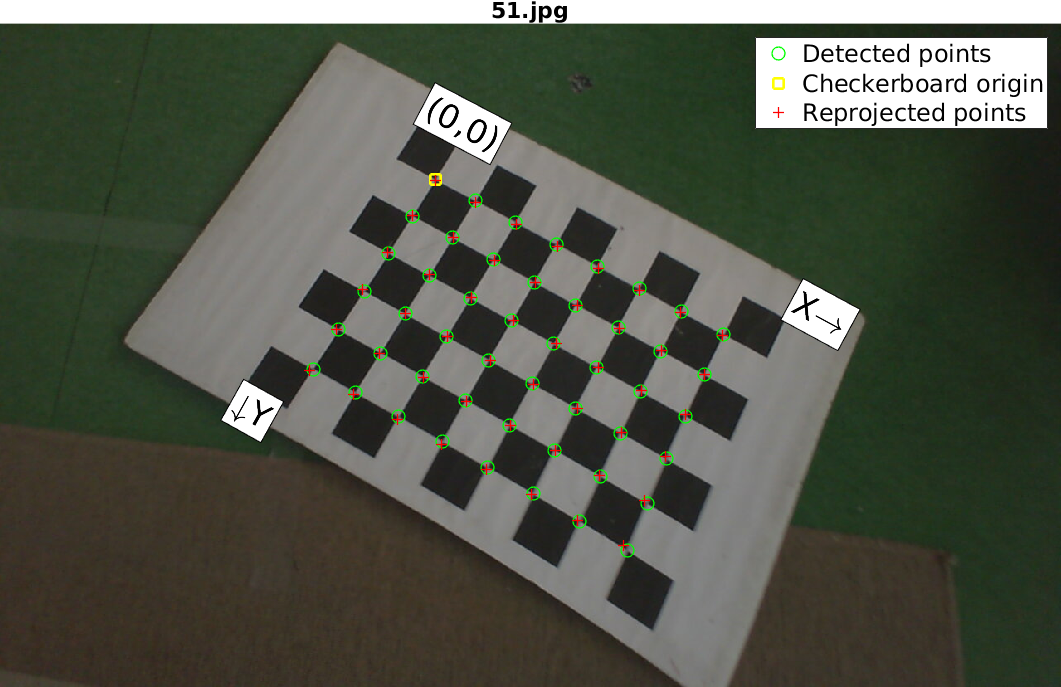
\includegraphics[width=0.7\textwidth]{graphics/worst.png}
\caption{Calibrated image with the highest amount of pixel error}
\label{fig:worst-calibrated-image}
\end{center}
\end{figure}

\begin{figure}[H]
\begin{center}
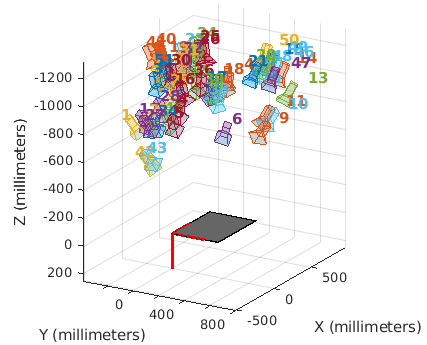
\includegraphics[width=0.7\textwidth]{graphics/camera_positions.png}
\caption{Camera positions evaluated via calibration procedure.}
\label{fig:poses}
\end{center}
\end{figure}

\begin{figure}[H]
\begin{center}
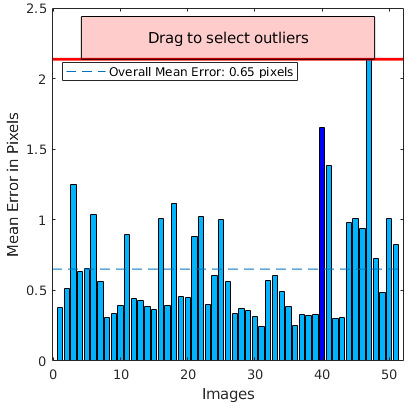
\includegraphics[width=0.7\textwidth]{graphics/stats.png}
\caption{Mean error in Pixels for each image.}
\label{fig:stats}
\end{center}
\end{figure}
\subsection*{2. Provide arguments for which camera model best fits your situation and hence should be used}

\subsection*{3. Discuss possible problems or error sources that can disturb the calibration process}
%%%%%%%%%%%%%%%%%%%%%%%%%%%%%%%%%%%%%%%%%%%%%%%%%%%%%%%%%%%%%%%%%%%%%%%%%%%%%